\section{infer}
\subsection{The confined Brownian motion}

We have seen that the bulk Brownian motion is well known and documented for a long time. But, in the real world, the boundaries are not at infinity and could play a role in the process of diffusion. Indeed, it was theorized by H. Faxen \cite{faxen_fredholm_1924} that the presence of a wall would change the Stokes-Einstein relation with a viscosity dependent to the position of the particle. As the particle get closer to a surface, the presence of the non-slip boundary condition make the fluid harder to push, thus increasing the local viscosity of the particle. This variation of the viscosity will be different for orthogonal and parallel displacement to the wall, thus we write respectively $\eta_\bot $ and $\eta_\parallel$ with $\eta_0$ being the fluid viscosity and $z$ the height of the particle:

\begin{equation}
	\eta_\bot = \frac{4}{3} \eta_0 \mathrm{sinh}\beta \sum _{n=1} ^{\infty} \frac{n(n+1)}{{2n-1}{2n+3}}
	\left[
	\frac
	{
		2\mathrm{sinh}(2n + 1)\beta + (2n +1)\mathrm{sinh}2\beta
	}
	{
		4\mathrm{sinh}^2(n + 1 /2)\beta  - (2n+1)^2 \mathrm{sinh}^2 \beta
	}
	-1
	\right] ~,
	\label{Eq:etaz}
\end{equation}

\nomenclature{$\eta_\bot$}{Viscosity orthogonal to a wall, see Eq.\ref{Eq:etaz}}
and 

\begin{equation}
	\eta_\parallel = \eta_0 
	\left[
	1 - \frac{9}{16} \xi + \frac{1}{8}\xi^3 - \frac{45}{256}\xi^4 - \frac{1}{16}\xi^5
	\right]^{-1}~,
	\label{Eq:etax}
\end{equation}
\nomenclature{$\eta_\parallel$}{Viscosity parrallel to a wall, see Eq.\ref{Eq:etax}}

where $\xi = \frac{a}{z+a}$ and $\beta = \mathrm{cosh}^{-1}(\xi)$. It is possible to simplify the form of $\eta_\bot$ by using a Padé approximation, which is correct up to $1\%$ of accuracy:

\begin{equation}
	\eta_\bot = \eta_0 \frac{6z^2 + 9az + 2a^2}{6z^2 + 2az}~.
\end{equation}

Of course, this local viscosity is directly reflected on the diffusive properties of the particle, hence a local diffusion coefficient, which we write:

\begin{equation}
	D_i (z) = \frac{k_\mathrm{B} T}{6\pi\eta_i (z) a}~.
\end{equation}

One of the first experimental measurement of the local diffusion coefficient was brought by Faucheux and Libchaber \cite{faucheux_confined_1994} where they measured the mean diffusion coefficient with various gaps and particle radius their results can be found in the Fig.\ref{fig:libchaber}.

\begin{figure}
	\centering
	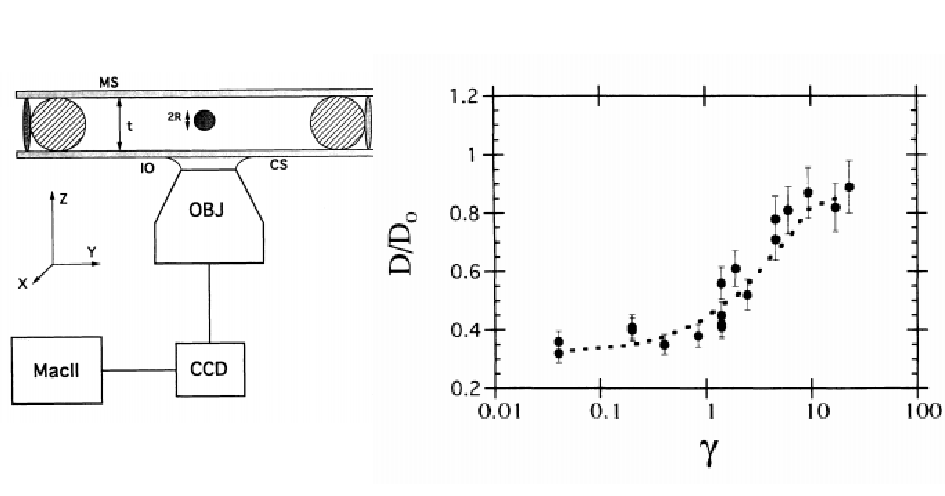
\includegraphics{02_body/chapter1/image/libchaber.pdf}
	\caption{Figure extracted from \cite{faucheux_confined_1994}, on the left is the experimental setup used. It is an inverted microscope used in order to track particle of size $2R$ inside a cell of thickness $t$. On the right is their final result, where they measure the diffusion parallel coefficient $D_\bot$ given by Eq.\ref{Eq:etax}, here normalized by $D_0$ the bulk diffusion coefficient as a function of  $\gamma$ a confinement constant $\gamma = (\langle z \rangle -a)/a$. }
	\label{fig:libchaber}
\end{figure}

Another interesting physical aspect to take into account when looking at confined Brownian motion is the potential the particle is lying into. Let's first consider the weight of the particle. Indeed, if the particle density does not match the fluid' one, a spherical particle will lye in a gravity potential given by:

\begin{equation}
	U_g(z) = \frac{4}{3} \pi a^3 (\rho_\mathrm{P} - \rho_\mathrm{F})gz~,
\end{equation}

\nomenclature{$g$}{Gravity constant}
\nomenclature{$\rho_\mathrm{P}$}{Particle density}
\nomenclature{$\rho_\mathrm{F}$}{Fluid density}

that we can rewrite for simplicity

\begin{equation}
	\frac{U_g(z)}{k_\mathrm{B} T} = \frac{z}{\ell_\mathrm{B}}~,
\end{equation}

\nomenclature{$\ell_\mathrm{B}$}{Boltzmann length}
with $\ell_\mathrm{B}$ the Boltzmann length which represents the balance between the kinetic energy and the weight of the particle:

\begin{equation}
	\ell_\mathrm{B} = \frac{k_\mathrm{B} T}{ \frac{4}{3} \pi a^3 \Delta \rho g}~.
\end{equation}

Let's now consider the interactions with the substrate, glass slides when immersed in water do charge negatively as well as polystyrene particles that we use. We will then have repulsive electrostatic interactions between the wall and the particles, the corresponding potential can be written as  \cite{israelachvili_intermolecular_2015}:

\begin{equation}
	\frac{U_\mathrm{elec}(z)}{k_\mathrm{B}T} = B \mathrm{e}^{-z/\ell_\mathrm{D}}~,
\end{equation}

\nomenclature{$B$}{Amplitude of the electrostatic interactions}
\nomenclature{$\ell_\mathrm{D}$}{Debye length}

where $B$ is the amplitude of electrostatic interactions, representing the surface charges and $\ell_\mathrm{D}$ being the Debye length, which is the characteristic length of the electrostatic interactions. The particle is thus lying in a total potential given by:

\begin{equation}
	\frac{U(z)}{k_\mathrm{B}T} =   B \mathrm{e}^{-z/\ell_\mathrm{D}} +  \frac{z}{\ell_\mathrm{B}}~.
\end{equation}

From this total potential one can construct the Gibbs-Boltzmann distribution in position:

\begin{equation}
	P_\mathrm{eq}(z) = A\mathrm{e}^
	{
		\frac{U}{k_\mathrm{B}T}	
	}~,
	\label{Eq:Peq}
\end{equation}

where $A$ is a normalization constant so that $\int P_\mathrm{eq} = 1$. This distribution gives us the probability to find the particle at a height $z$. The exponential decay due to the gravity was first measured by Perrin \cite{perrin_les_2014} by methodically counting through a microscope the number of colloids in suspension as a function on the height. 


\begin{figure}[ht]
	\centering
	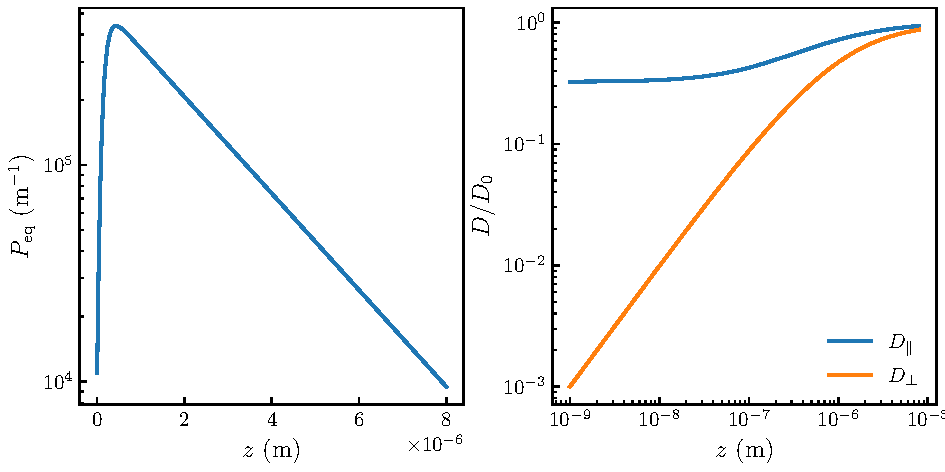
\includegraphics{02_body/chapter1/image/theorie_chap1.pdf}
	\caption{On the left, plot of the Gibbs-Boltzmann distribution Eq.\ref{Eq:Peq} for $a = 1 ~ \mathrm{\mu m}$, $ B = 4 $, $\ell _\mathrm{D} = 100 ~ \mathrm{nm}$ and $\Delta \rho = 50 ~ \mathrm{kg.m^{-3}}$. On the right, local diffusion coefficient normalized by bulk diffusion coefficient $D_0 = k_\mathrm{B}T/\gamma$, given by Eq.\ref{Eq:etax} and Eq.\ref{Eq:etaz}}.
\end{figure}